\section{Resultados}

\subsection{Resposta em Frequência (AC) e Análise de Polos e Zeros}

A magnitude linear da tensão de saída $V_{\text{out}}$ (\texttt{/net10}), obtida por meio da simulação AC, está representada na Figura~\ref{fig:ac_mag_lin}. Com essa análise, foi possível observar a característica \textit{equiripple} da aproximação de Chebyshev de quinta ordem ($N=5$), evidenciada pelos cinco picos máximos de aproximadamente $500\text{ mV}$ ($499{,}63\text{ mV}$ em $6{,}267\text{ GHz}$ e $499{,}42\text{ mV}$ em $6{,}743\text{ GHz}$) dentro da banda passante ($6{,}25\text{ GHz}$ a $6{,}75\text{ GHz}$). Esse valor corresponde à metade da amplitude da fonte ($1\text{ V}$), comprovando a ausência de perdas dissipativas nos elementos reativos ideais e o casamento de impedância entre $R_0 = 50~\Omega$ e $R_L = 50~\Omega$.

\begin{figure}[!htbp]
    \centering
    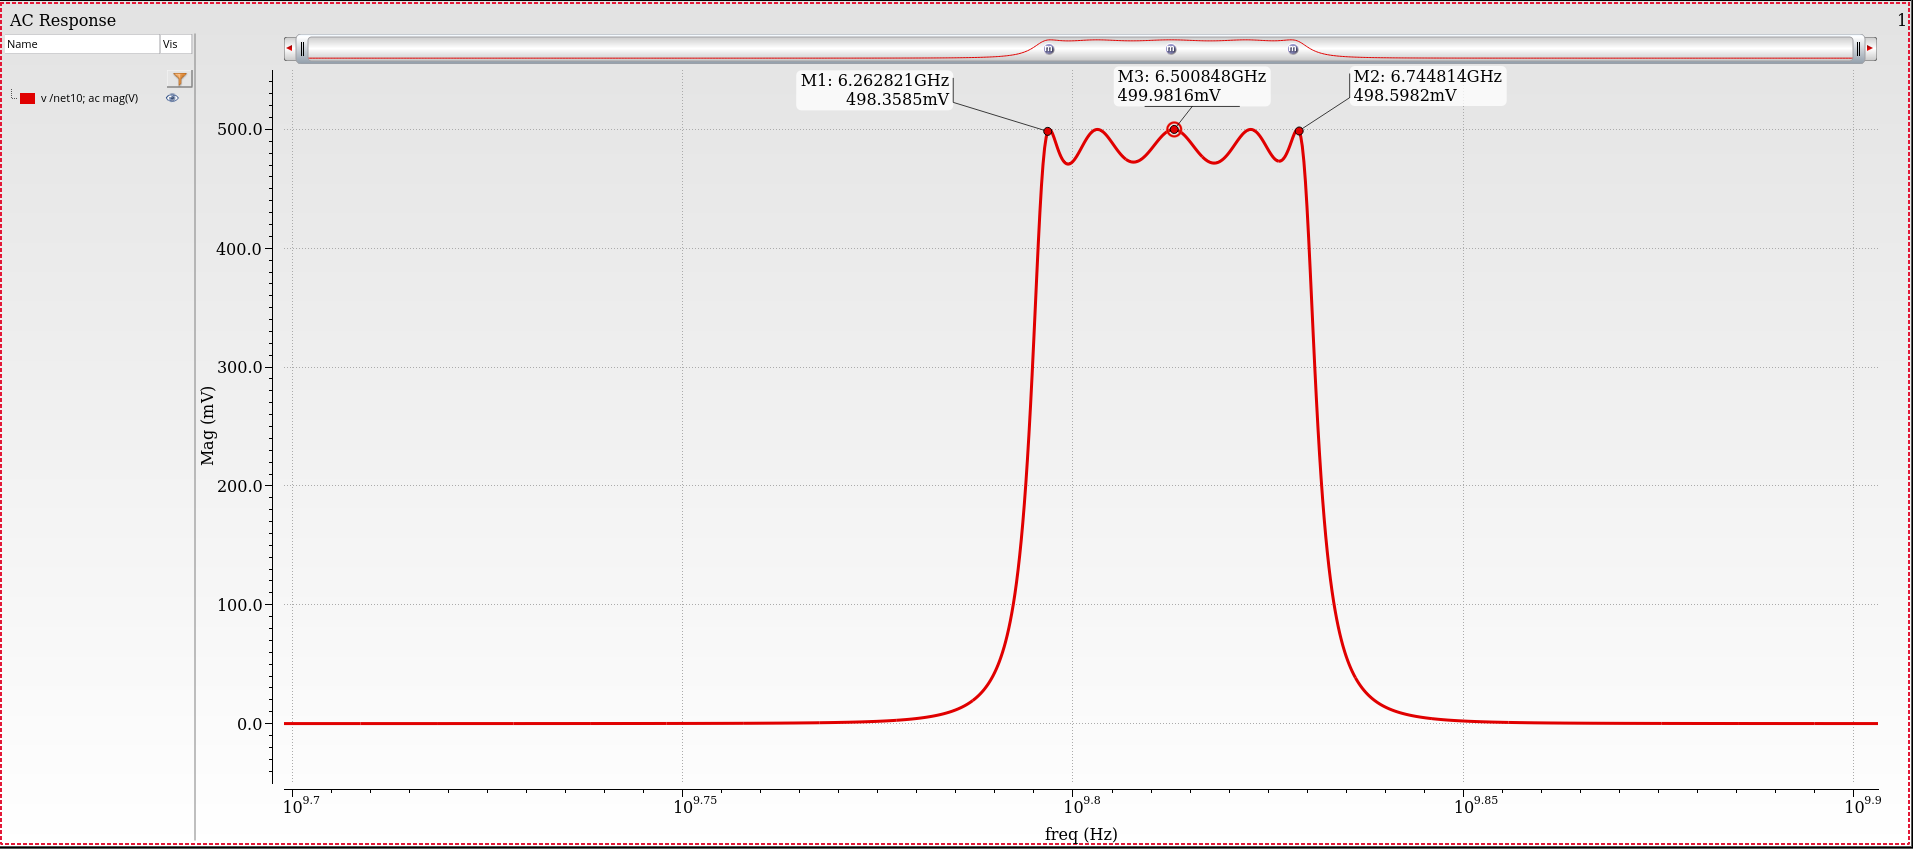
\includegraphics[width=0.95\linewidth]{Results/Fig/ac_mag_lin.png}
 \caption{Magnitude linear em $\text{mV}$ da resposta em frequência AC no nó \texttt{/net10}, que mostra os cinco ripples de Chebyshev na banda passante.}

    \label{fig:ac_mag_lin}
\end{figure}

Na curva em decibéis (Figura~\ref{fig:ac_mag_db}), o patamar máximo estabiliza em $-6{,}02\text{ dB}$ em $f_0 = 6{,}50\text{ GHz}$ devido ao divisor resistivo natural de $1/2$ ($20\log_{10}(0{,}5)$) formado pelas terminações de fonte e carga, apresentando ondulação interna limitada ao \textit{ripple} projetado de $0{,}5\text{ dB}$ (com mínimo de $-6{,}54\text{ dB}$ na borda inferior em $6{,}254\text{ GHz}$ e $-6{,}12\text{ dB}$ sobre a crista final em $6{,}748\text{ GHz}$, imediatamente antes da queda abrupta na borda superior de $6{,}75\text{ GHz}$, cujo mínimo teórico é $-6{,}52\text{ dB}$). Fora da banda passante, a atenuação acentua-se rapidamente, atingindo cerca de $25\text{ dB}$ de rejeição relativa nas bordas da especificação de largura total $1{,}5 \times BW$ ($6{,}125\text{ GHz}$ e $6{,}875\text{ GHz}$) e ultrapassando $40\text{ dB}$ em afastamentos de $\pm 500\text{ MHz}$ da portadora ($6{,}0\text{ GHz}$ e $7{,}0\text{ GHz}$), atendendo integralmente ao requisito mínimo de $25\text{ dB}$ do roteiro \cite{Filter1}.

\begin{figure}[!htbp]
    \centering
    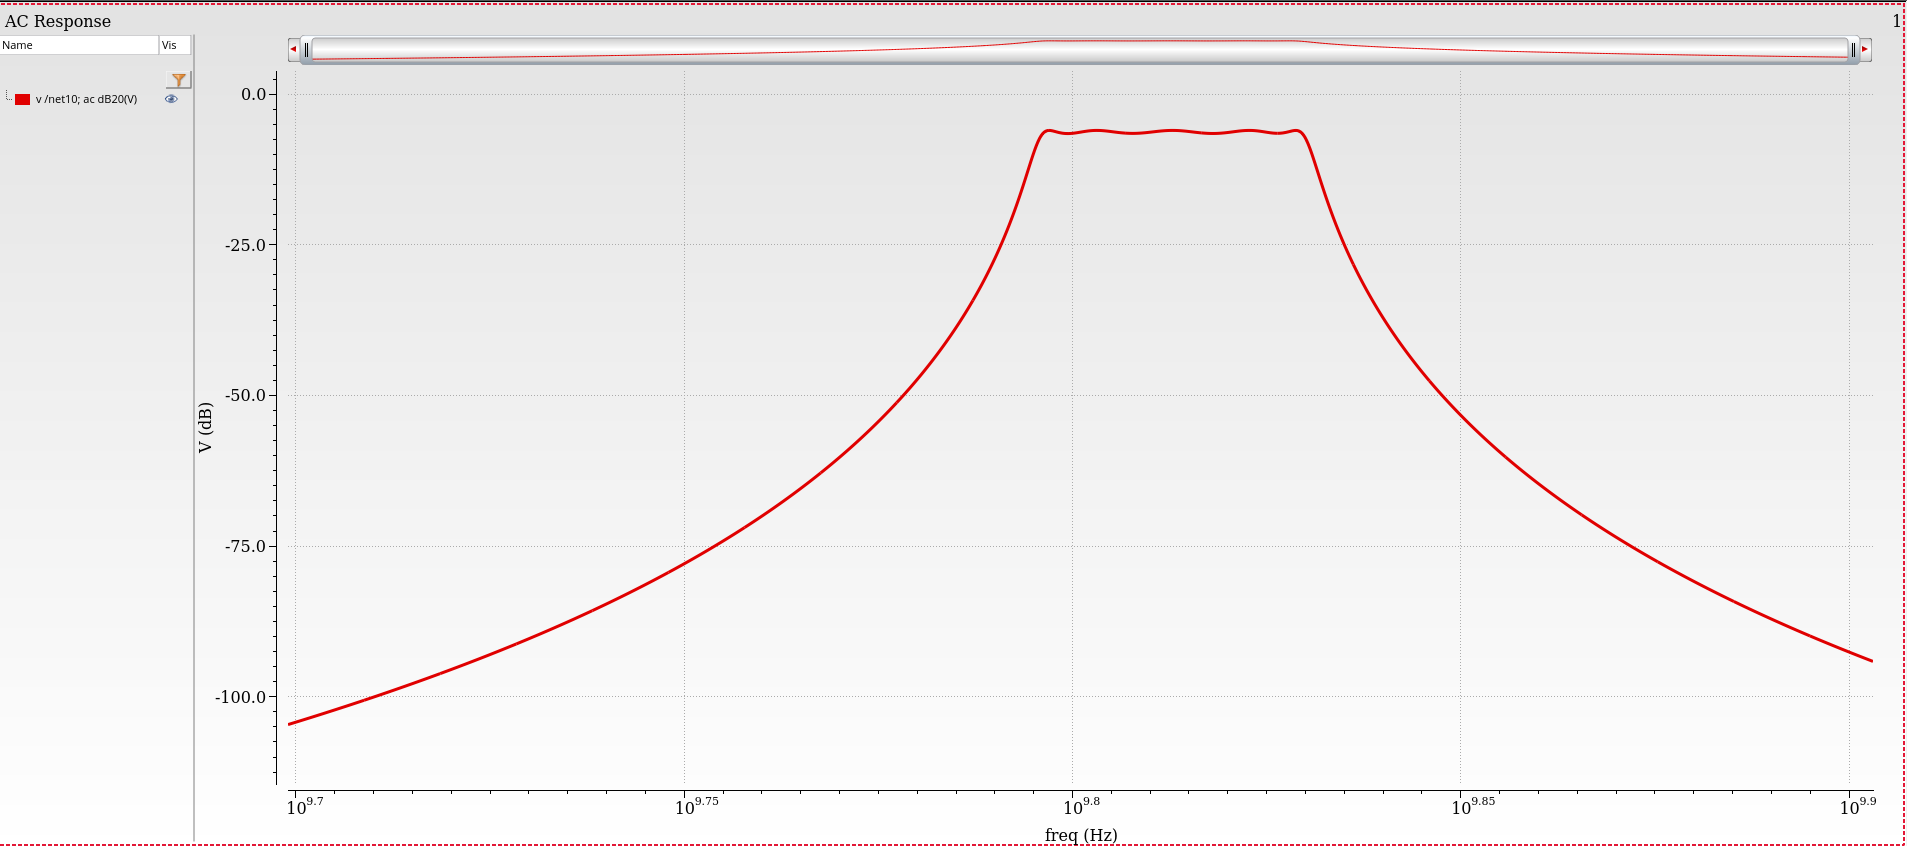
\includegraphics[width=0.95\linewidth]{Results/Fig/ac_mag_db.png}
    \caption{Magnitude em $\text{dB20}$ da resposta em frequência AC no nó \texttt{/net10}, destacando os marcadores de corte e o patamar de $-6{,}02\text{ dB}$.}
    \label{fig:ac_mag_db}
\end{figure}

A resposta de fase de $V_{\text{out}}$ (Figura~\ref{fig:ac_phase}) exibe comportamento monotônico e aproximadamente linear na região central da banda passante, cruzando $-363{,}88^\circ$ na frequência central de $6{,}504\text{ GHz}$. Ao longo da varredura de $5\text{ GHz}$ a $8\text{ GHz}$ (representada em eixo logarítmico, onde $10^{9{,}813}\text{ Hz} \approx 6{,}5\text{ GHz}$), observa-se uma excursão de fase de aproximadamente $872{,}6^\circ$ (de $+77{,}80^\circ$ em $5{,}255\text{ GHz}$ até $-794{,}85^\circ$ em $7{,}726\text{ GHz}$), tendendo assintoticamente aos $900^\circ$ ($10 \times 90^\circ$) esperados para os dez polos do sistema.

\begin{figure}[!htbp]
    \centering
    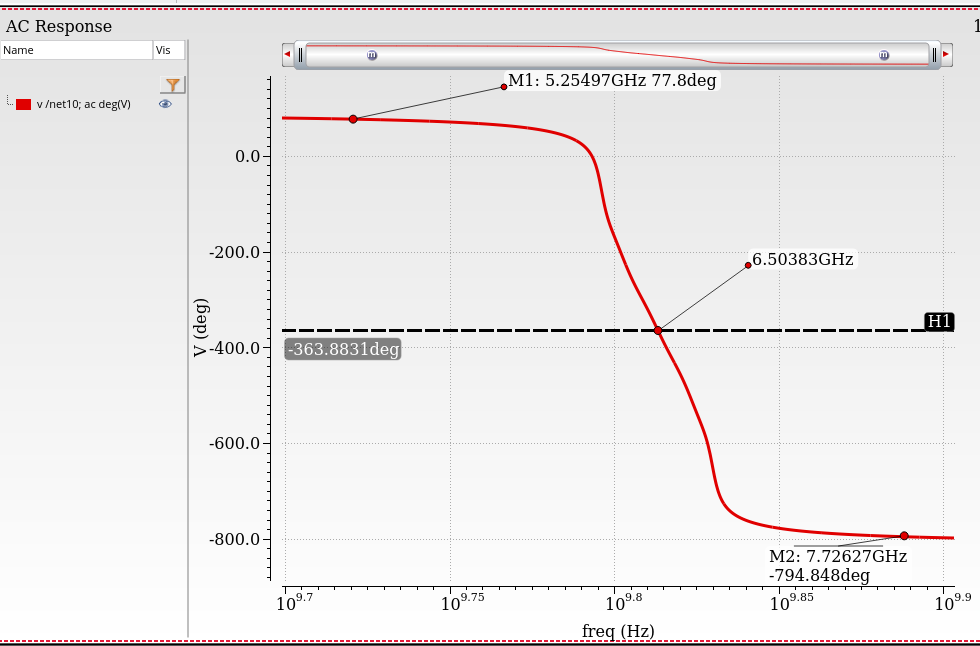
\includegraphics[width=0.95\linewidth]{Results/Fig/ac_phase.png}
    \caption{Resposta de fase em graus da tensão de saída \texttt{/net10} na simulação AC.}
    \label{fig:ac_phase}
\end{figure}

A distribuição de polos e zeros no plano complexo $s$ confirma a síntese analítica do filtro. Como esperado para uma transformação passa-faixa de quinta ordem, o circuito apresenta $10$ polos divididos em cinco pares complexos conjugados no semiplano esquerdo ($\text{Re}(s) < 0$, Figura~\ref{fig:pz_poles}), garantindo estabilidade incondicional. Os polos mais próximos do eixo imaginário situam-se nas bordas da banda passante ($6{,}252\text{ GHz}$ com $\sigma = -26{,}74\text{ MHz}$ e $6{,}757\text{ GHz}$ com $\sigma = -29{,}23\text{ MHz}$), sendo fisicamente responsáveis pela transição abrupta nas frequências de corte. Simultaneamente, o diagrama de zeros (Figura~\ref{fig:pz_zeros}) evidencia o zero na origem ($0\text{ Hz}$, de multiplicidade $N=5$ decorrente da transformação passa-faixa), assegurando o bloqueio completo de componentes DC.

\begin{figure}[!htbp]
    \centering
    \begin{minipage}[t]{0.48\linewidth}
        \centering
        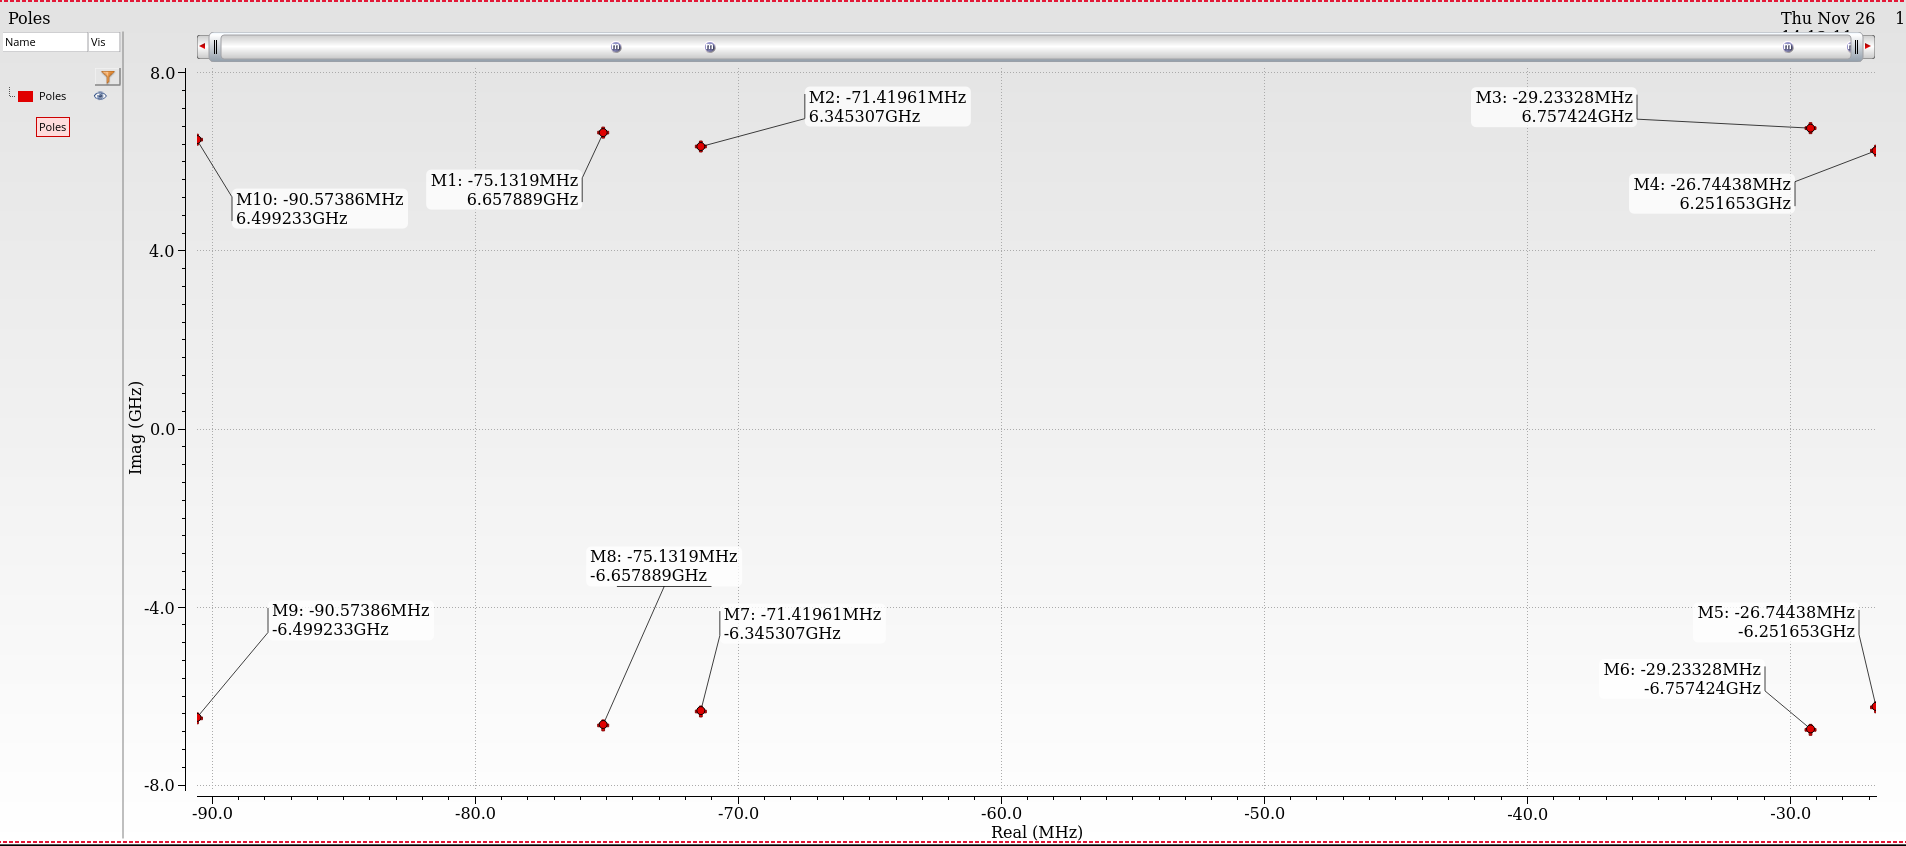
\includegraphics[width=\linewidth]{Results/Fig/pz_poles.png}
        \caption{Diagrama de polos no plano complexo $s$ ($6{,}25\text{ GHz}$ a $6{,}75\text{ GHz}$).}
        \label{fig:pz_poles}
    \end{minipage}
    \hfill
    \begin{minipage}[t]{0.48\linewidth}
        \centering
        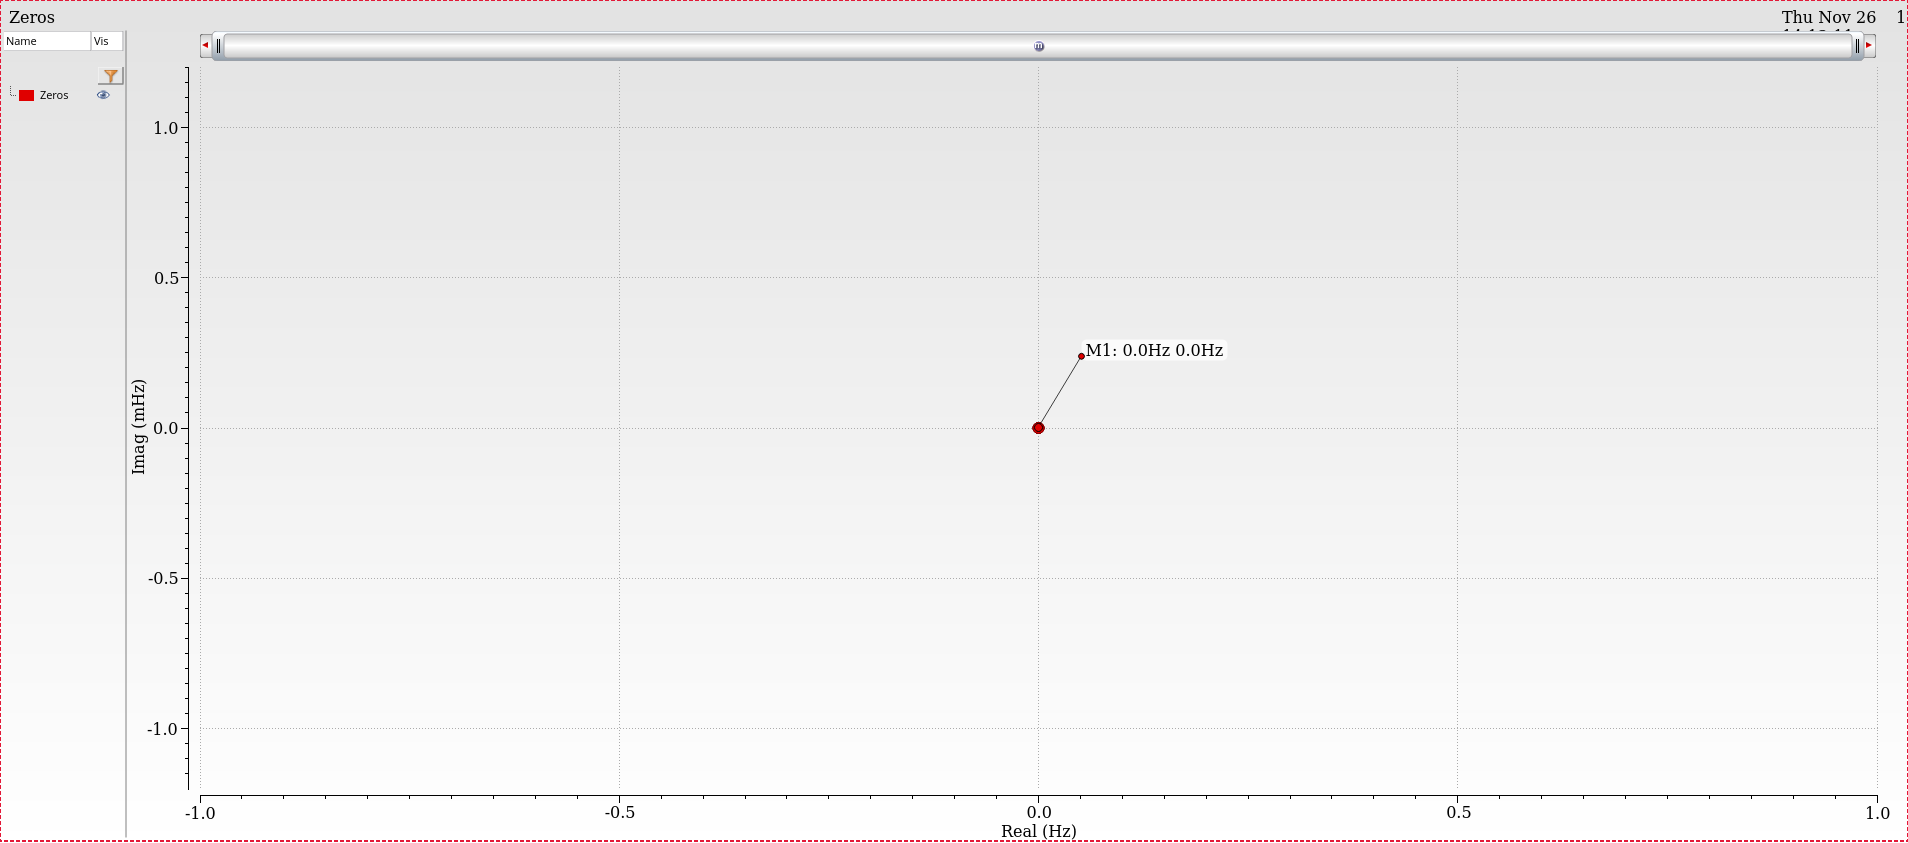
\includegraphics[width=\linewidth]{Results/Fig/pz_zeros.png}
        \caption{Diagrama de zeros no plano $s$ (multiplicidade $5$ na origem).}
        \label{fig:pz_zeros}
    \end{minipage}
\end{figure}

\subsection{Análise de Parâmetros de Espalhamento (SP)}

A caracterização de potência por parâmetros de espalhamento ratifica o desempenho de transmissão e casamento de impedância do filtro. Na resposta em banda larga de $5\text{ GHz}$ a $8\text{ GHz}$ (Figura~\ref{fig:sp_full}), a curva de transmissão direta $S_{21}$ atinge $0{,}00\text{ dB}$ ($-30{,}55~\mu\text{dB}$) na frequência central de $6{,}50\text{ GHz}$, confirmando perda de inserção (\textit{insertion loss}) nula para componentes ideais (variando até $0{,}50\text{ dB}$ nos vales do \textit{ripple} dentro da banda passante), enquanto a atenuação fora da banda alcança $-98{,}60\text{ dB}$ em $5{,}0\text{ GHz}$ e $-87{,}89\text{ dB}$ em $8{,}0\text{ GHz}$. Simultaneamente, devido à reciprocidade da rede passiva sem perdas, o coeficiente de transmissão reversa $S_{12}$ exibe comportamento idêntico a $S_{21}$.

\begin{figure}[!htbp]
    \centering
    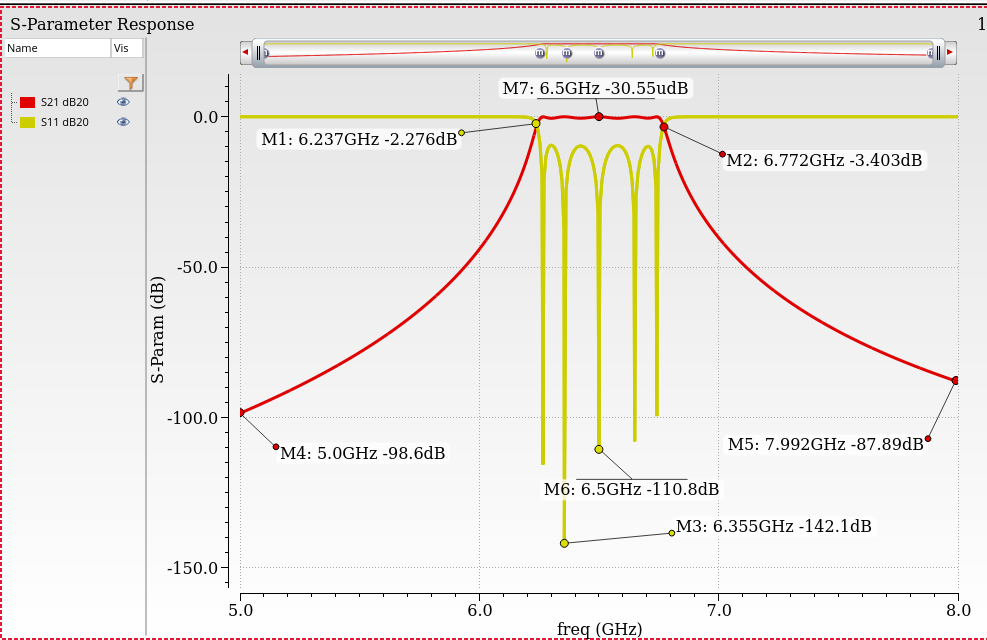
\includegraphics[width=0.95\linewidth]{Results/Fig/sp_s21_s11_full.png}
    \caption{Parâmetros de espalhamento $S_{21}$ e $S_{11}$ em $\text{dB20}$ de $5\text{ GHz}$ a $8\text{ GHz}$, evidenciando os cinco polos de reflexão na banda passante e a atenuação fora da banda.}
    \label{fig:sp_full}
\end{figure}

O coeficiente de reflexão na entrada ($S_{11}$) apresenta cinco vales profundos de casamento (atingindo $-142{,}15\text{ dB}$ em $6{,}355\text{ GHz}$ e $-110{,}84\text{ dB}$ em $6{,}50\text{ GHz}$), refletindo a simetria física da topologia também observada no coeficiente de reflexão de saída $S_{22}$ (Figura~\ref{fig:sp_s22}). Fora da banda passante, tanto $S_{11}$ quanto $S_{22}$ aproximam-se de $0\text{ dB}$, indicando que a potência dos sinais indesejados é refletida de volta à fonte em vez de ser dissipada internamente.

\begin{figure}[!htbp]
    \centering
    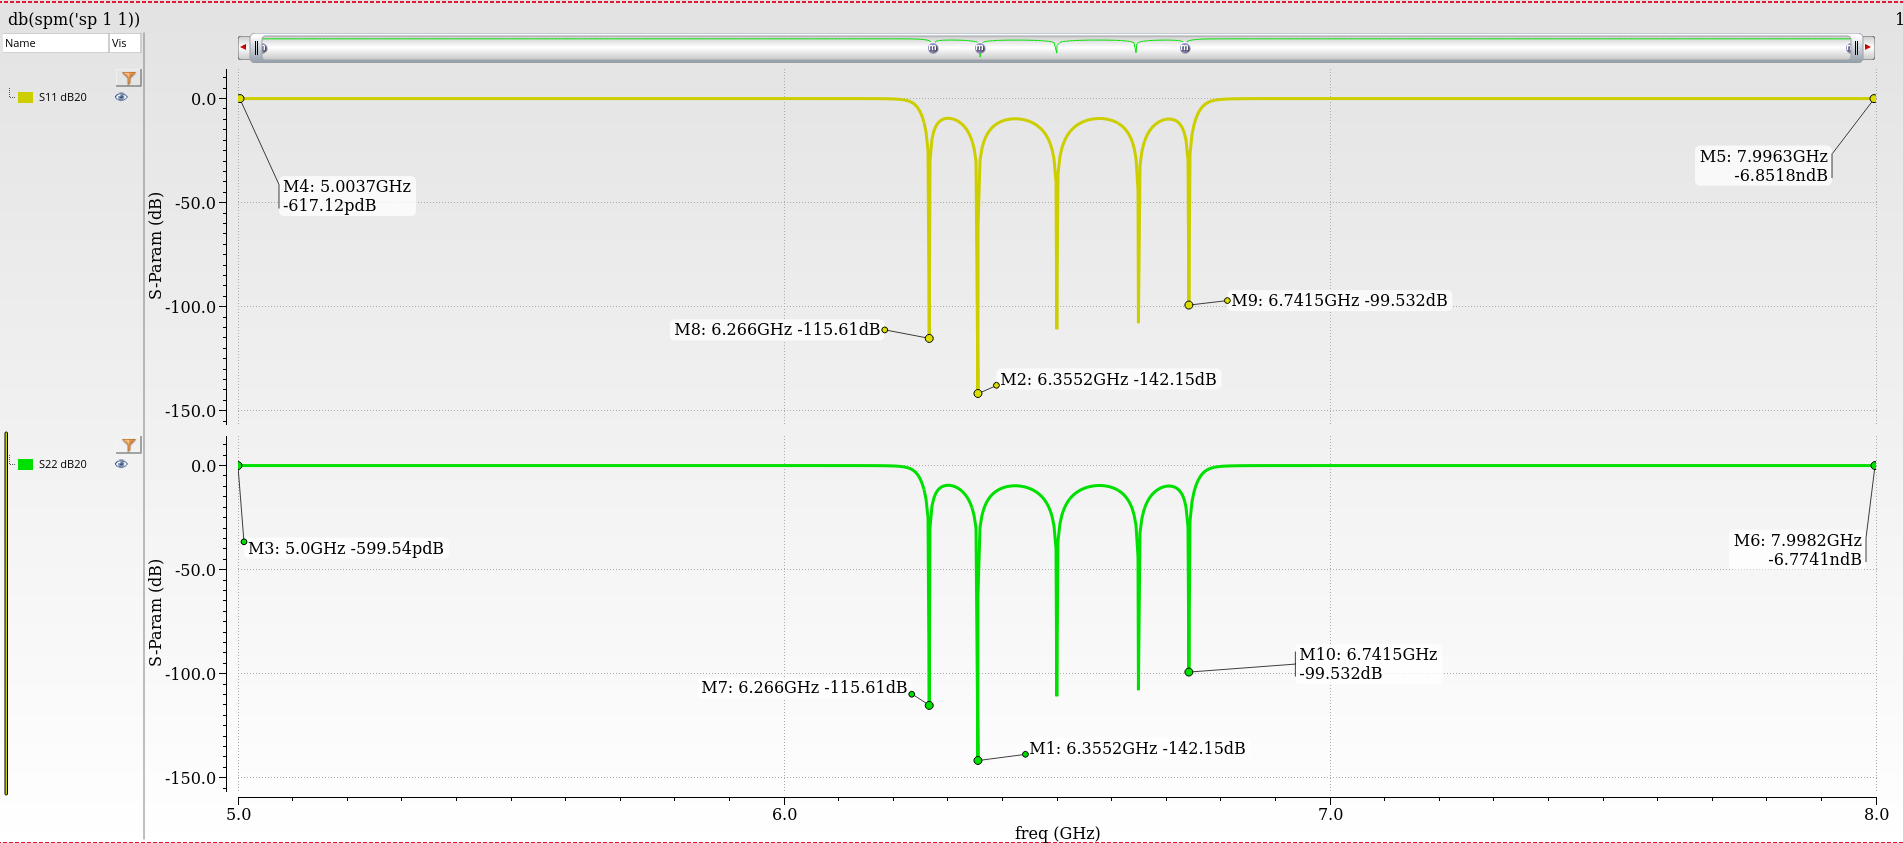
\includegraphics[width=0.95\linewidth]{Results/Fig/sp_s22.png}
    \caption{Coeficiente de reflexão na porta de saída ($S_{22}$) em $\text{dB20}$, comprovando a simetria da rede em relação a $S_{11}$.}
    \label{fig:sp_s22}
\end{figure}

No detalhamento da banda passante entre $6{,}0\text{ GHz}$ e $7{,}0\text{ GHz}$ (Figura~\ref{fig:sp_zoom}), observa-se que os arcos máximos de reflexão $S_{11}$ entre os vales de casamento limitam-se a aproximadamente $-9{,}64\text{ dB}$, valor teoricamente esperado para um \textit{ripple} de $0{,}5\text{ dB}$ ($|S_{11}|_{\max} = \sqrt{1 - 10^{-0{,}05}} \approx 0{,}3296$, equivalente a uma perda de retorno mínima de $9{,}64\text{ dB}$). Nos limites da faixa de rejeição especificada ($1{,}5 \times BW$ total), a transmissão direta $S_{21}$ atinge $-28{,}36\text{ dB}$ em $6{,}125\text{ GHz}$ e $-25{,}05\text{ dB}$ em $6{,}875\text{ GHz}$, cumprindo o critério mínimo de $25\text{ dB}$ de atenuação em ambos os lados da banda.

\begin{figure}[!htbp]
    \centering
    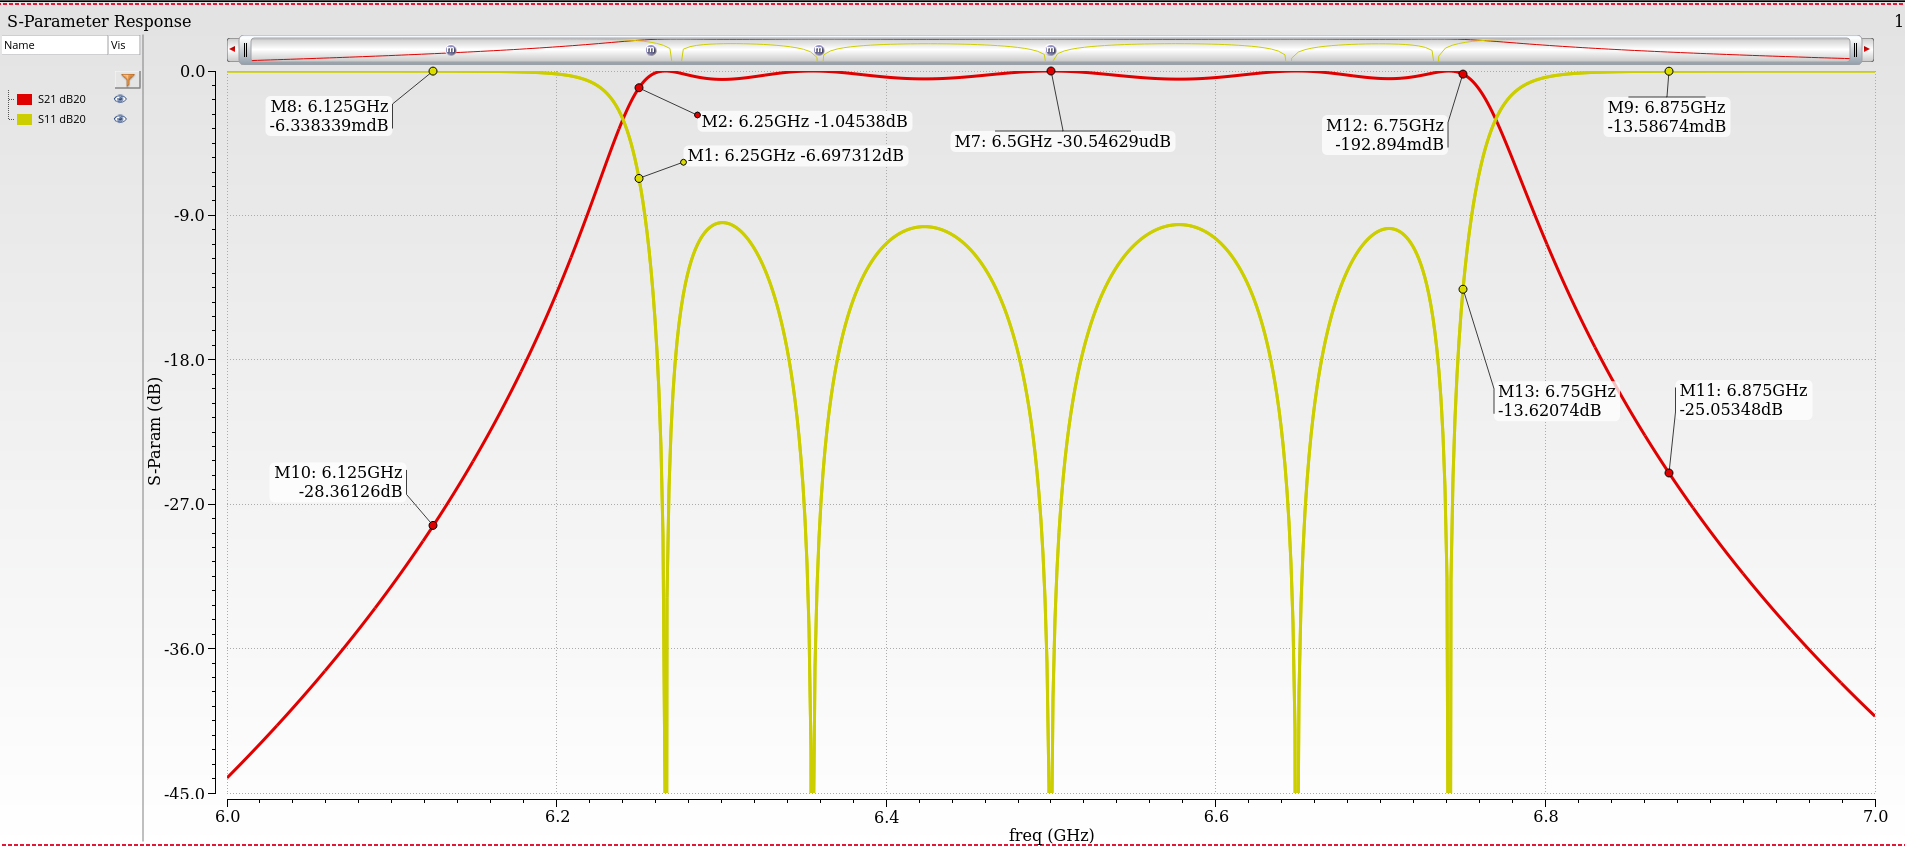
\includegraphics[width=0.95\linewidth]{Results/Fig/sp_zoom.png}
    \caption{Detalhe dos parâmetros $S_{21}$ e $S_{11}$ entre $6{,}0\text{ GHz}$ e $7{,}0\text{ GHz}$, destacando o \textit{ripple} na banda passante, o limite superior de $S_{11}$ ($\approx -9{,}64\text{ dB}$) e os pontos de atenuação em $6{,}125\text{ GHz}$ e $6{,}875\text{ GHz}$.}
    \label{fig:sp_zoom}
\end{figure}

A resposta de fase de $S_{21}$ (Figura~\ref{fig:sp_phase}) exibe variação monotônica e aproximadamente linear na região central da banda passante (cruzando $-360{,}19^\circ$ em $6{,}50\text{ GHz}$), característica desejável para minimizar a distorção de atraso de grupo ($\tau_g = -\mathrm{d}\phi/\mathrm{d}\omega$) no centro do canal, apresentando inclinação mais acentuada apenas próximo às frequências de corte. Entre $5{,}0\text{ GHz}$ e $8{,}0\text{ GHz}$, a fase varia de $+80{,}12^\circ$ até $-797{,}49^\circ$, perfazendo uma excursão total de $877{,}61^\circ$, coerente com a assíntota teórica de $900^\circ$ ($10 \times 90^\circ$) associada aos dez polos do filtro.

\begin{figure}[!htbp]
    \centering
    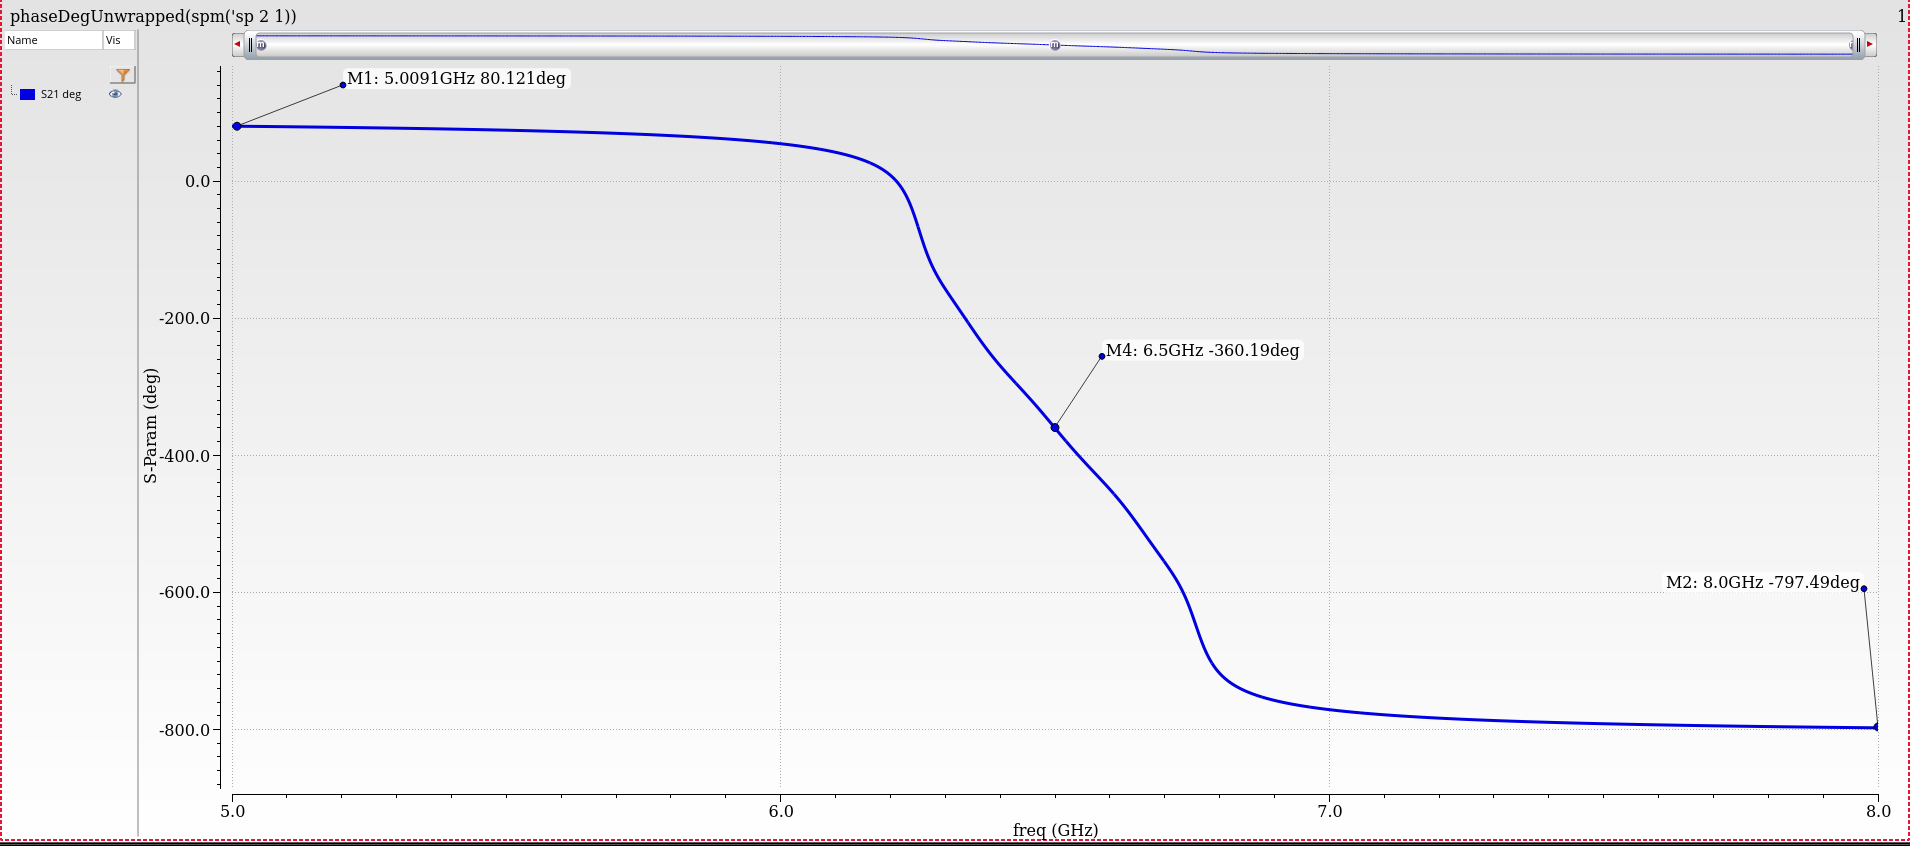
\includegraphics[width=0.95\linewidth]{Results/Fig/sp_phase.png}
    \caption{Resposta de fase do parâmetro $S_{21}$ em graus de $5\text{ GHz}$ a $8\text{ GHz}$.}
    \label{fig:sp_phase}
\end{figure}

A Tabela~\ref{tab:resumo_specs} consolida a comparação entre os requisitos de projeto e os valores medidos nas simulações lineares.

\begin{table}[!htbp]
\centering
\caption{Comparação entre as especificações do projeto e os resultados simulados (AC e SP).}
\label{tab:resumo_specs}
\setlength{\tabcolsep}{3pt}
\resizebox{\linewidth}{!}{%
\begin{tabular}{lccc}
\hline
\textbf{Parâmetro} & \textbf{Especificado} & \textbf{Simulado} & \textbf{Status} \\
\hline
Frequência central ($f_0$) & $6{,}50\text{ GHz}$ & $6{,}50\text{ GHz}$ & Atendido \\
Largura de banda ($BW$) & $500\text{ MHz}$ & $500\text{ MHz}$ & Atendido \\
Impedância terminal ($Z_0$) & $50~\Omega$ & $50~\Omega$ & Atendido \\
\textit{Ripple} na banda passante & $\le 1{,}0\text{ dB}$ & $0{,}50\text{ dB}$ & Atendido \\
Perda de inserção ($IL_{\min}$) & Ideal ($0\text{ dB}$) & $0{,}00\text{ dB}$ & Atendido \\
Perda de retorno mínima ($RL_{\min}$) & --- & \begin{tabular}[c]{@{}c@{}}$9{,}64\text{ dB}$\\($|S_{11}| \le -9{,}64\text{ dB}$)\end{tabular} & Coerente \\
Atenuação em $6{,}125 / 6{,}875\text{ GHz}$ ($1{,}5 \times BW$) & $\ge 25\text{ dB}$ & $28{,}36\text{ dB} / 25{,}05\text{ dB}$ & Atendido \\
Atenuação em $6{,}00 / 7{,}00\text{ GHz}$ ($f_0 \pm 500\text{ MHz}$) & $\ge 25\text{ dB}$ & $> 40\text{ dB}$ & Atendido \\
\hline
\end{tabular}%
}
\end{table}

\subsection{Avaliação Não Linear e Rejeição de Banda Adjacente (HB e Envelope)}

Para avaliar a rejeição a produtos de intermodulação e interferentes adjacentes gerados por não linearidades, analisou-se inicialmente o espectro multi-tom por balanço harmônico (\texttt{hb\_mt}) com a portadora útil em $f_1 = 6{,}5\text{ GHz}$ e um tom interferente em $f_2 = 6{,}0\text{ GHz}$ excitando o amplificador de potência (\texttt{PA\_PB}, ganho de $27{,}2\text{ dB}$ e $P_{1\text{dB}} = 5\text{ dBm}$). Conforme ilustrado na Figura~\ref{fig:hb_espectro} e quantificado na Tabela~\ref{tab:hb_mt}, a não linearidade cúbica do PA gera produtos de intermodulação de terceira ordem ($IM_3$) em $2f_1 - f_2 = 7{,}0\text{ GHz}$ e $2f_2 - f_1 = 5{,}5\text{ GHz}$. Na saída do filtro (\texttt{/net10}), a portadora útil em $6{,}5\text{ GHz}$ é preservada sem atenuação ($-6{,}38\text{ dBV}$ antes e após o filtro), enquanto o interferente em $6{,}0\text{ GHz}$ sofre rejeição de $49{,}66\text{ dB}$ e os produtos $IM_3$ em $7{,}0\text{ GHz}$ e $5{,}5\text{ GHz}$ são atenuados em $45{,}73\text{ dB}$ e $84{,}29\text{ dB}$, respectivamente.

\begin{figure}[!htbp]
    \centering
    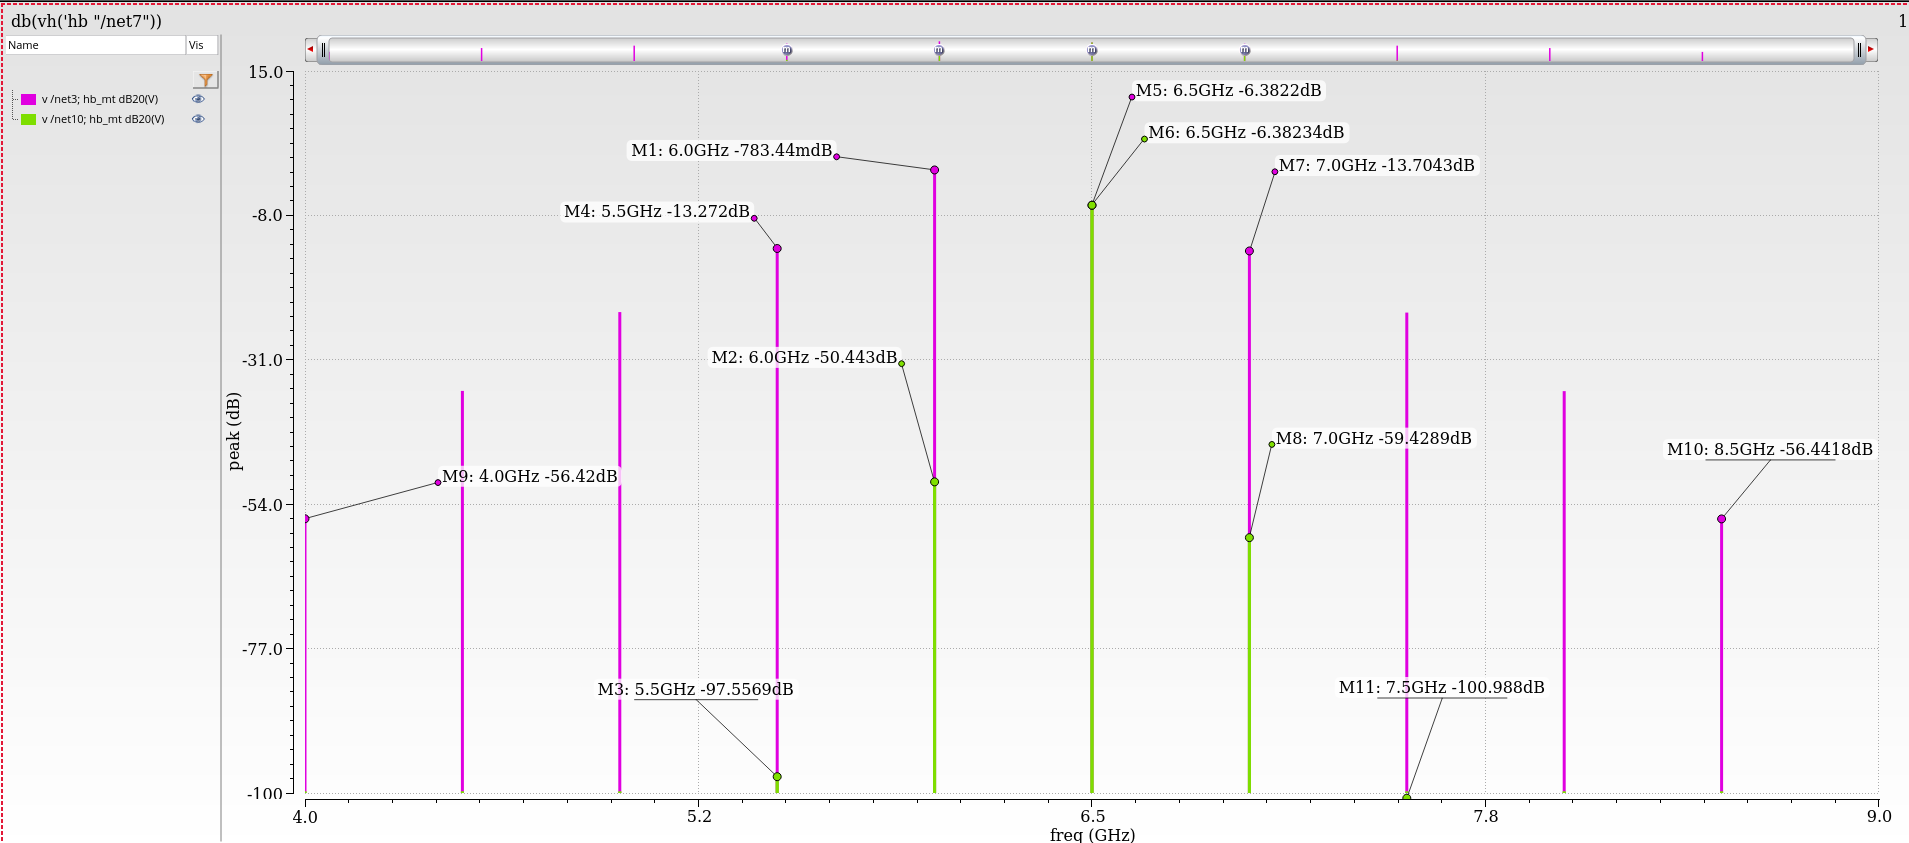
\includegraphics[width=\linewidth]{Results/Fig/hb_espectro.png}
    \caption{Espectro multi-tom (\texttt{hb\_mt}) na saída do PA (\texttt{/net3}, magenta) e após o filtro passa-faixa (\texttt{/net10}, verde), destacando a preservação do tom em $6{,}5\text{ GHz}$ e a supressão de $49{,}66\text{ dB}$ em $6{,}0\text{ GHz}$.}
    \label{fig:hb_espectro}
\end{figure}

\begin{table}[!htbp]
    \centering
    \caption{Níveis de tensão espectral antes e após o filtro na análise multi-tom (\texttt{hb\_mt}).}
    \label{tab:hb_mt}
    \resizebox{\linewidth}{!}{%
    \begin{tabular}{lccc}
        \hline
        \textbf{Componente Espectral} & \textbf{Pós-PA (\texttt{/net3})} & \textbf{Pós-Filtro (\texttt{/net10})} & \textbf{Rejeição (dB)} \\
        \hline
        Portadora útil ($6{,}5\text{ GHz}$) & $-6{,}38\text{ dBV}$ & $-6{,}38\text{ dBV}$ & $0{,}00\text{ dB}$ \\
        Interferente adjacente ($6{,}0\text{ GHz}$) & $-0{,}78\text{ dBV}$ & $-50{,}44\text{ dBV}$ & $49{,}66\text{ dB}$ \\
        Produto $IM_3$ superior ($7{,}0\text{ GHz}$) & $-13{,}70\text{ dBV}$ & $-59{,}43\text{ dBV}$ & $45{,}73\text{ dB}$ \\
        Produto $IM_3$ inferior ($5{,}5\text{ GHz}$) & $-13{,}27\text{ dBV}$ & $-97{,}56\text{ dBV}$ & $84{,}29\text{ dB}$ \\
        \hline
    \end{tabular}%
    }
\end{table}

Na sequência, realizou-se a análise de envelope (\texttt{envlp}) com o sinal modulado OFDM 16-QAM em $6{,}5\text{ GHz}$ (Figura~\ref{fig:psdacpr}). O sinal de entrada (\texttt{WPRB0}) apresenta potência média de $-0{,}04\text{ dBm}$ ($-36{,}61\text{ mdBm}$) e razão de potência no canal adjacente (ACPR) de $-65{,}79\text{ dBc}$ (inferior) e $-65{,}73\text{ dBc}$ (superior). Ao atravessar o amplificador de potência operando próximo à região de compressão ($P_{\text{in}} = 0\text{ dBm}$, $P_{1\text{dB}} = 5\text{ dBm}$), a potência média no canal eleva-se para $5{,}42\text{ dBm}$ (\texttt{WPRB1}) e o alargamento espectral (\textit{spectral regrowth}) degrada o ACPR em $\pm 40\text{ MHz}$ para $-19{,}69\text{ dBc}$ e $-19{,}71\text{ dBc}$. Na saída do filtro (\texttt{WPRB2}), o ACPR medido em $\pm 40\text{ MHz}$ permanece em $-18{,}56\text{ dBc}$ e $-18{,}54\text{ dBc}$, pois esse afastamento situa-se integralmente dentro da banda passante de $500\text{ MHz}$ ($\pm 250\text{ MHz}$ em torno de $6{,}5\text{ GHz}$), enquanto a rejeição atua sobre produtos de intermodulação e interferentes afastados ($\ge 375\text{ MHz}$ da portadora). A pequena diferença de $+0{,}13\text{ dB}$ na potência média integrada em \texttt{WPRB2} ($5{,}55\text{ dBm}$) decorre da integração numérica da PSD na janela da sonda aliada ao descasamento reativo entre a saída do PA e a impedância do filtro fora da banda.

\begin{figure}[!htbp]
    \centering
    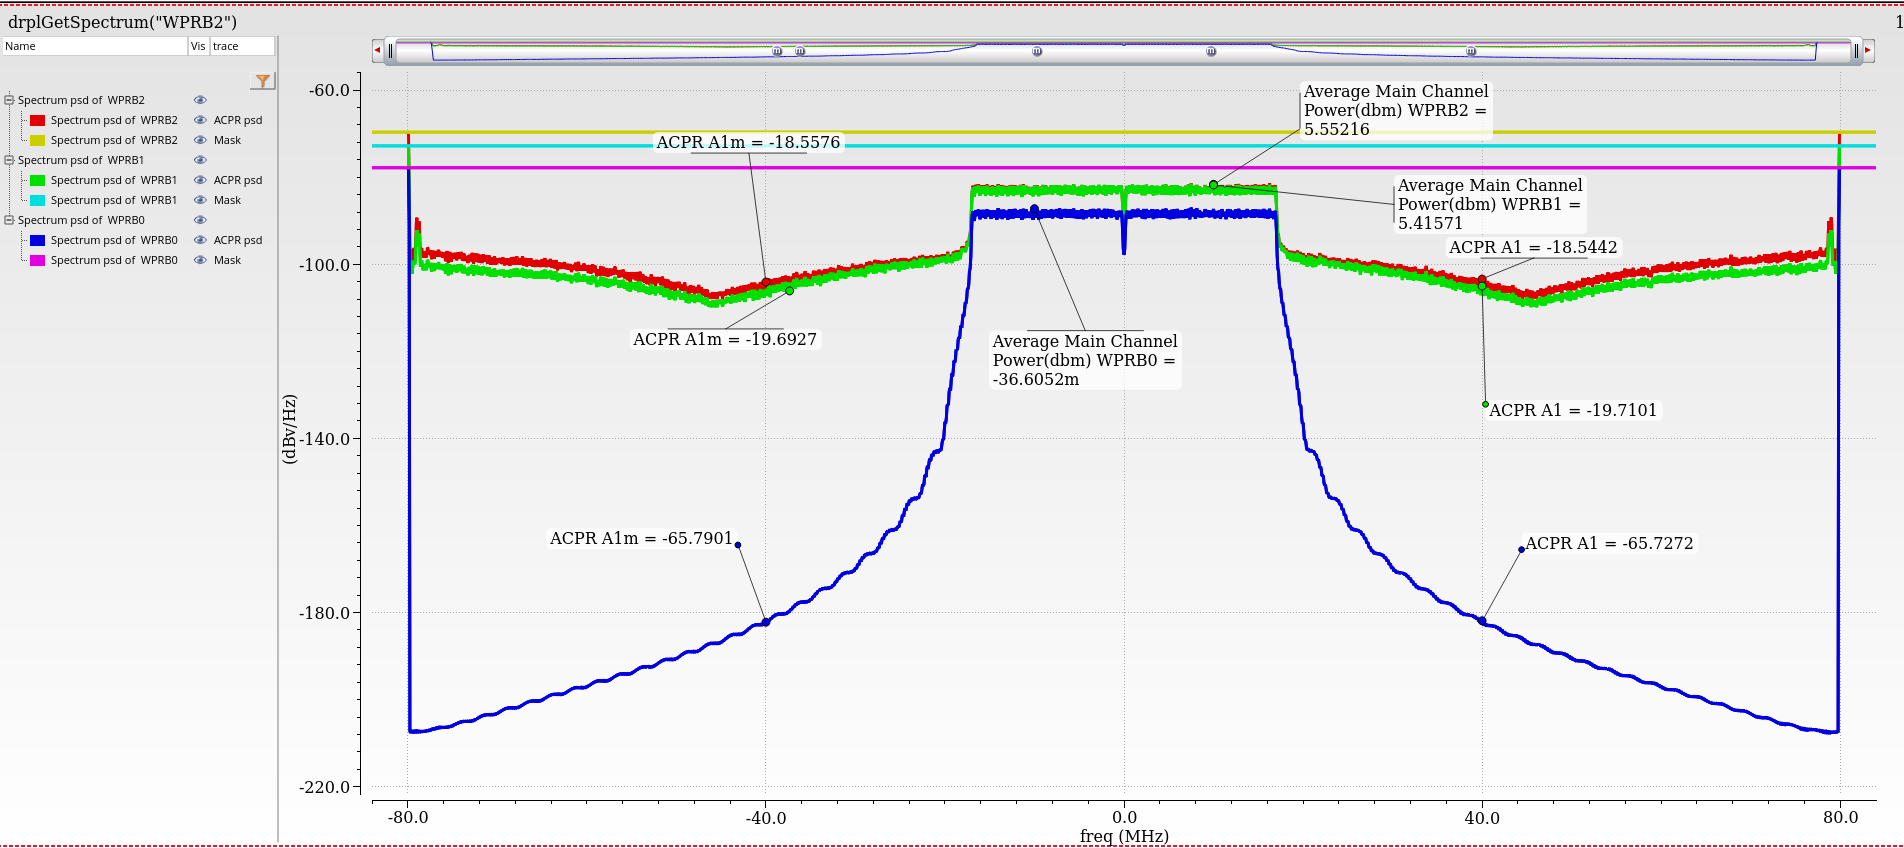
\includegraphics[width=\linewidth]{Results/Fig/PSD e ACPR.png}
    \caption{Densidade Espectral de Potência (PSD) e Razão de Potência no Canal Adjacente (ACPR) nas sondas \texttt{WPRB0}, \texttt{WPRB1} e \texttt{WPRB2}.}
    \label{fig:psdacpr}
\end{figure}

No domínio da potência, confirma-se a compressão dos picos de envoltória responsável pelo espalhamento espectral, conforme ilustrado pelas curvas de CCDF na Figura~\ref{fig:CCDF}. O sinal OFDM original (\texttt{WPRB0}) exibe relação pico-média (PAPR) de até $10{,}92\text{ dB}$, valor que é reduzido para $7{,}84\text{ dB}$ após o ceifamento no amplificador (\texttt{WPRB1}) e para $3{,}11\text{ dB}$ na saída do filtro (\texttt{WPRB2}), refletindo o corte das componentes espectrais de alta frequência responsáveis pelos transientes rápidos de envoltória.

\begin{figure}[!htbp]
    \centering
    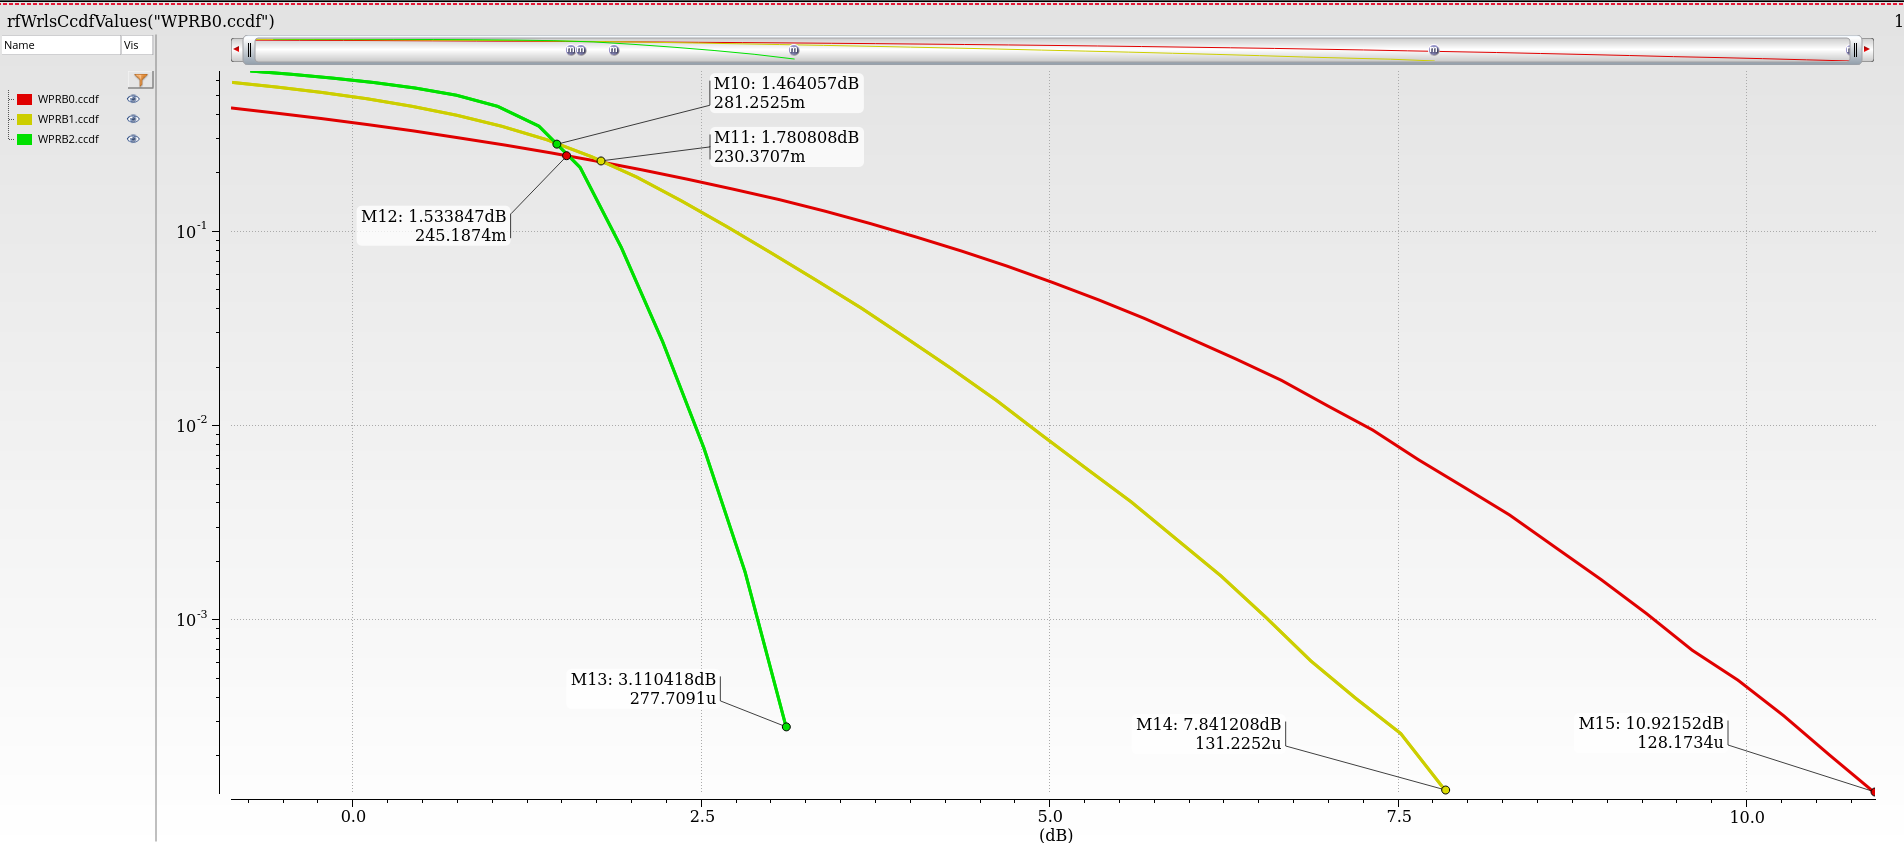
\includegraphics[width=\linewidth]{Results/Fig/CCDF.png}
    \caption{Função de Distribuição Cumulativa Complementar (CCDF) do sinal nas sondas \texttt{WPRB0}, \texttt{WPRB1} e \texttt{WPRB2}.}
    \label{fig:CCDF}
\end{figure}

No domínio da modulação, a comparação entre o sinal gerado pela fonte e o sinal distorcido após o amplificador está representada nas Figuras~\ref{fig:const_wprb0} e~\ref{fig:const_wprb1}, enquanto a Tabela~\ref{tab:nonlinear} consolida todas as métricas extraídas nas três sondas. Na entrada (\texttt{WPRB0}), os $16$ símbolos apresentam erro residual desprezível ($\mathrm{EVM} = 0{,}03\%$ e $\mathrm{BER} = 0\%$). Após a saturação do amplificador (\texttt{WPRB1}), as distorções não lineares de amplitude e fase (AM-AM e AM-PM) dispersam os símbolos da constelação, elevando o $\mathrm{EVM}$ para $28{,}10\%$ e a $\mathrm{BER}$ para $4{,}88\%$. Na saída do filtro (\texttt{WPRB2}), a atenuação de componentes espúrias fora da banda reduz parcialmente o erro para $\mathrm{EVM} = 23{,}74\%$ e $\mathrm{BER} = 2{,}58\%$, demonstrando fisicamente que o filtro suprime interferências e harmônicas externas, mas não corrige distorções geradas dentro da própria banda passante.

\begin{figure}[!htbp]
    \centering
    \begin{subfigure}[b]{0.8\linewidth}
        \centering
        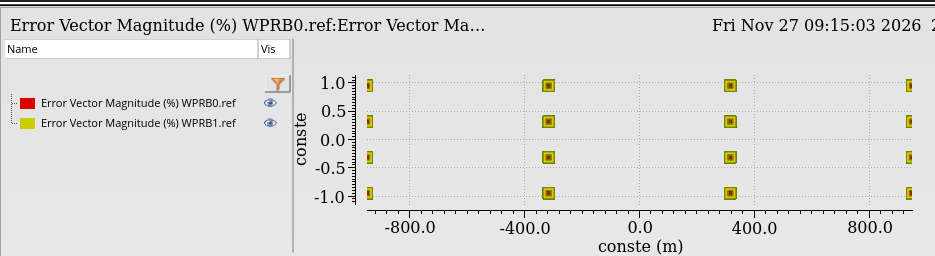
\includegraphics[width=\linewidth]{Results/Fig/Constelação 16-QAM 3.png}
        \caption{Saída da fonte (\texttt{WPRB0}, $\text{EVM} = 0{,}03\%$).}
        \label{fig:const_wprb0}
    \end{subfigure}
    
    \vspace{0.4cm}
    
    \begin{subfigure}[b]{0.8\linewidth}
        \centering
        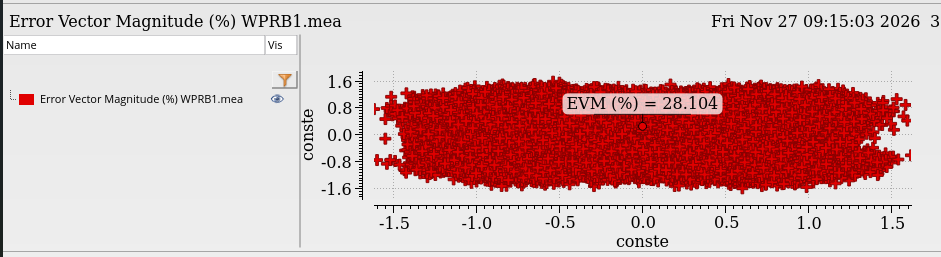
\includegraphics[width=\linewidth]{Results/Fig/Constelação 16-QAM 2.png}
        \caption{Pós-PA (\texttt{WPRB1}, $\text{EVM} = 28{,}10\%$).}
        \label{fig:const_wprb1}
    \end{subfigure}
    \caption{Constelações 16-QAM e medidas de EVM.}
    \label{fig:constelacoes_qam}
\end{figure}


\begin{table}[!htbp]
    \centering
    \caption{Resumo das métricas não lineares e de modulação obtidas na simulação de envelope.}
    \label{tab:nonlinear}
    \resizebox{\linewidth}{!}{%
    \begin{tabular}{lccc}
        \hline
        \textbf{Métrica} & \textbf{WPRB0 (Fonte)} & \textbf{WPRB1 (Pós-PA)} & \textbf{WPRB2 (Pós-Filtro)} \\
        \hline
        Potência Média no Canal & $-0{,}04\text{ dBm}$ & $5{,}42\text{ dBm}$ & $5{,}55\text{ dBm}$ \\
        ACPR Inferior / Superior & $-65{,}79 / -65{,}73\text{ dBc}$ & $-19{,}69 / -19{,}71\text{ dBc}$ & $-18{,}56 / -18{,}54\text{ dBc}$ \\
        PAPR Máximo (CCDF) & $10{,}92\text{ dB}$ & $7{,}84\text{ dB}$ & $3{,}11\text{ dB}$ \\
        Taxa de Erro de Bit (BER) & $0\%$ & $4{,}88\%$ & $2{,}58\%$ \\
        EVM (\%) & $0{,}03\%$ & $28{,}10\%$ & $23{,}74\%$ \\
        \hline
    \end{tabular}%
    }
\end{table}